\chapter[Better Documenting Computer Vision Services]
{Better Documenting Computer Vision Services\pubfootnote{Cummaudo:2020tse}}
\label{ch:tse2020}
\graphicspath{{mainmatter/publications/figures/tse2020/}}

\def\circlenotpresent{\faCircleO}
\def\circlepartialpresent{\faAdjust}
\def\circlepresent{\faCircle}
\newcommand{\dimcat}[1]{\textsc{\small[\textbf{#1}]}}

% Taxonomy Dimension Keys
\def \dima{Usage Description}
\def \dimb{Design Rationale}
\def \dimc{Domain Concepts}
\def \dimd{Support Artefacts}
\def \dime{Documentation Presentation}

% Suggested improvements
\def\SuggestedImprovement{\noindent\itshape\small\textbf{\faHandORight{} Suggested improvement:~}}

\glsresetall
\begin{abstract}
Using cloud-based \glspl{cvs} is gaining traction with developers for many applications for many reasons: developers can simply access these AI-components through familiar RESTful \glsacpl{api}, and need not orchestrate large training and inference infrastructures or curate and label large training datasets.
However, while their \glsacpl{api} \textit{seem} familiar to use, their non-deterministic run-time behaviour and evolution profile are not adequately communicated to developers, and this results in developers struggling to use such \glsacpl{api} in-practice.
Therefore, improving these services' \glsac{api} documentation is paramount, as a more complete document facilities the development process of intelligent software.
This study presents an analysis of what facets a `complete' \glsac{api} document should have, as synthesised into a taxonomy from 21 academic studies via a systematic mapping study. We triangulate these findings from literature against 83 developers to assess the efficacy and utility in-practice of such knowledge. We produce two weighted `scores' for each dimension in our taxonomy based on (i) the number of papers producing these outcomes and their citation count and (ii) the extent to which developers \textit{agree} with the recommendations arising from these studies (based on our survey).
Furthermore, we apply the taxonomy to three popular \glspl{cvs} and assess their compliance, producing a third `score' using the taxonomy to identify 12 suggested improvements to the \glsac{api} documentation of these \glslongpl{iws}.
\end{abstract}
\glsresetall

\section{Introduction}

Improving \glsac{api} documentation quality is a valuable task for any \glsac{api}---an extensive \glsac{api} document facilitates productivity, and therefore improved quality is better engineered into a system~\citep{mcleod2011factors}. Where application developers integrate new services (such as \glspl{cvs}~\citep{Cummaudo:2019icsme}) into their systems via \glsacpl{api}, their productivity is affected either by inadequate skills (\textit{``I've never used an \glsac{api} like this, so must learn from scratch''}) or, where their skills are adequate, an imbalanced cognitive load that causes excessive context switching (\textit{``I have the skills for this, but am confused or misunderstand''}). This is commonly seen in the emerging \gls{cv} web services space, where the documentation does not yet completely or correctly describe the \glsacpl{api} in full~\citep{Cummaudo:2020icse}. 

What causes a developer to be confused and how to mitigate it via an improved \glsac{api} document has been largely explored for conventional \glsacpl{api}. Various studies have provided a myriad of recommendations based on both qualitative and quantitative analysis of developer opinion. Such recommendations propose ways by which developers, managers and solution architects can construct systems better with improved documentation. However, while previous works have covered certain aspects of \glsac{api} usage, many have lacked a systematic review of literature and do not offer a taxonomy to consolidate these guidelines together. For example, some studies have considered the technical implementation improving \glsac{api} usability or tools to generate (or validate) \glsac{api} documentation from its source code (e.g.,~\citep{Nybom:2018ef,Watson:2012uy,Maalej2013}); still lacks a consolidated effort to capture recommendations on how to \textit{manually write} complete, correct, and effective \glsac{api} documentation. The works that \textit{do} produce these recommendations from literature are largely scattered across multiple sources, and systematically capturing the information into a readily accessible, consolidated framework (designed to assist writing \glsac{api} documentation) must be validated in real-world circumstances to assess its efficacy with practitioners and existing documentation~\citep{Cummaudo:2019esem}.

As a real-world use case, consider an \gls{iws}---such as \glspl{cvs}---in which an AI-based component produces a non-deterministic result based on a machine-learnt data-driven algorithm, rather than a predictable, rule-driven one~\citep{Cummaudo:2019icsme}. These services use machine intelligence to make predictions on images such as object labelling or facial recognition~\citepweb{GoogleCloud:Home,AWS:Home,Azure:Home,IBM:Home,Pixlab:Home,Clarifai:Home,Cloudsight:Home,DeepAI:Home,Imagaa:Home,Talkwaler:Home,Megvii:Home,TupuTech:Home,YiTuTech:Home,SenseTime:Home,DeepGlint:Home}. The impacts of poor and incomplete documentation results in developer complaints on online discussion forums such as Stack Overflow~\citep{Cummaudo:2020icse}. Many comments show that developers do not think in the non-deterministic mental model of the designers who created the \glspl{cvs}. They ask many varied questions from their peers to try and clarify their understanding.

This paper significantly extends our previous work~\citep{Cummaudo:2019esem} by evaluating our \glsac{api} documentation taxonomy in two additional contexts. In our previous work, we developed a weighted metric for each dimension and category based on how many literary sources agree that the aspects of our taxonomy should be implemented. We refer to this as an `in-literature' agreement score. We build upon this facet but \textit{in-practice} by assessing the efficacy of our taxonomy against developers using a survey built upon an interpretation of the \gls{sus}~\citep{Brooke:1996ua}. We produce a second weighting for the dimensions and categories of the taxonomy, referred to as a `in-practice' agreement score. We then compare both the in-literature and in-practice scores directly, thereby contrasting the statistical agreement the two have. Lastly, we assess the taxonomy against three popular \glspl{cvs}, namely Google Cloud Vision~\citepweb{GoogleCloud:Home}, Amazon Rekognition~\citepweb{AWS:Home} and Azure Computer Vision~\citepweb{Azure:Home}. For each category in our taxonomy, we assess whether the respective service's documentation contains, partially-contains or does not contain the recommendation. From this, we triangulate each category's in-literature and in-practice score against the service's level of inclusion of the recommendation, thereby making a judgement as to where the services can improve their documentation to make them more complete.

The primary contributions in this work are:

\begin{itemize}
  \item a \gls{sms} consisting of 21 studies that capture what knowledge or artefacts should be contained within \glsac{api} documentation;
  \item a five dimensional taxonomy consisting of 34 recommendations based on those consolidated from the 21 studies;
  \item a score metric for each recommendation based on the number of papers that agree with the recommendation;
  \item a score metric assessing the efficacy of the 34 recommendations that empirically reflects what is important to document from a \textit{practitioner} point of view; and,
  \item a heuristic validation of each recommendation against \glspl{cvs}, assessing where existing \gls{cvs} \glsac{api} documentation needs improvement.
\end{itemize}

After performing our \gls{sms} on what \glsac{api} knowledge should be captured in documentation to assist \glsac{api} designers, we propose our taxonomy consisting of the following dimensions: (1)~\dima{}; (2)~\dimb{}; (3)~\dimc{}; (4)~\dimd{}; and (5)~\dime{}. Following this, we adopted the \gls{sus} surveying technique to assess the overall utility of each of these recommendations, producing a survey consisting of 43 questions. This survey was then tested three times within our research group: firstly against three researchers for feedback on the survey's design, secondly against three software engineers in our research group with varying levels of experience for developers for test-retest reliability~\citep{Kitchenham:2007ux}, thirdly against 22 software engineers in our research group for wider feedback on the survey. Given these feedback improvements, we surveyed 83 external developers between May 2019 to October 2019, and then analysed the relevance of each recommendation from the practitioner's viewpoint. We also assessed the three \glspl{cvs} for inclusion of each recommendation, and once our surveys were complete, determined a weighted `score' of each service to see where improvements to their documentation was made.

This paper is structured as thus: \cref{tse2020:sec:related-work} presents related work in the areas of \glsac{api} usability, intelligent \glspl{cvs}, and the \gls{sus}; \cref{tse2020:sec:method} is divided into two subsections, the first describing how primary sources were selected in a \gls{sms} with the second describing the development of our taxonomy from these sources; \cref{tse2020:sec:findings} presents the taxonomy; \cref{tse2020:sec:validation} describes how we developed a survey instrument of 43 questions to validate the taxonomy against developers, and assess its efficacy against the three popular \glspl{cvs} selected to make 12 suggested improvements to the existing service \glsac{api} documentation; \cref{tse2020:sec:tax-analysis} presents the findings from our validation analysis and the weightings for the taxonomy; \cref{tse2020:sec:limitations} describes the threats to validity of this work and \cref{tse2020:sec:conclusions} provides concluding remarks and the future directions of this study. Additional materials are provided in \cref{ch:tse-supplementary-materials}.

\section{Related Work}
\label{tse2020:sec:related-work}



\subsection{\glsac{api} Usability and Documentation Knowledge}

Use of the \gls{sms} approach has explored developer experience and \glsac{api} usability. A~\citeyear{Nybom:2018ef} study reviewed 36 \glsac{api} documentation generation tools and approaches, and analysed the tools developed and their inputs and documentation outputs~\citep{Nybom:2018ef}. The findings from this study emphasise that the largest effort in \glsac{api} documentation tooling is to assist developers to generate either example code snippets and/or templates or natural language descriptions of the \glsac{api} directly from the program's source code. These snippets or descriptions can then be placed in the \glsac{api} documentation, thereby increasing the efficiency at which \glsac{api} documentation can be written. Additionally, tools from 12 studies target the maintainability of existing \glsacpl{api} of existing \glsacpl{api}, with tools from 11 studies target the correctness and accuracy of the documentation by validating that what is written in the documentation is accurate to the technical structure of the \glsac{api}. From the end-developer's perspective, some tools (17 studies) help target improvements to the developer's understandability and learnability of new \glsacpl{api} by linking in examples directly with questions such as on Stack Overflow.

However, the results from this study regards the \textit{tooling} used to either assist in producing, validating or learning from \glsac{api} documentation. While this is a systematic study with key insights into the types of tooling produced, there is still a gap for a \gls{sms} in what \textit{guidelines} have been produced by the literature in developing natural-language documentation itself and how well developers \textit{agree} to those guidelines, which our work has addressed.

\citet{Watson:2012uy} performed a heuristic assessment from 35 popular \glsacpl{api} against 11 high-level universal design elements of \glsac{api} documentation. This study highlighted how many \glsacpl{api}, even popular ones, fail to grasp these basic design elements. For example, 25\% of the documentation sets did not provide any basic overview documentation to the \glsac{api}. The heuristics used within~\citeauthor{Watson:2012uy}'s study is based on only three seminal works and only contains 11 design elements---our study extends these heuristics and structures them into a consolidated, hierarchical taxonomy which we then validate against practitioners.

A taxonomy of distinct knowledge patterns within reference documentation by~\citet{Maalej2013} classified 12 distinct knowledge types. The taxonomy was then evaluated against the JDK 6 and .NET 4.0 frameworks, and showed that the functionality and structure of these \glsacpl{api} are well-communicated, although core concepts and rationale about the \glsac{api} are quite rarer to see. The authors also identified low-value `non-information'---described as documentation that provides uninformative boilerplate text with no insight into the \glsac{api} at all---which was  substantially present in the documentation of methods and fields in the two frameworks. They recommend that developers factor their 12 distinct knowledge types into the process of code documentation, thereby preventing low-value non-information. The development of their taxonomy consisted of questions to model knowledge and information, thereby capturing the reason about disparate information units independent to context; a key difference to this paper is the systematic taxonomy approach utilised.


\subsection{Adapting the System Usability Scale}

The \gls{sus} was first introduced by~\citeauthor{Brooke:1996ua} as early as 1986 as a ``quick and dirty'' survey scale to easily assess the overall usability of a product or service in a timely manner. Its popularity in the usability community demonstrated the need for a tool that can collect a quantifiable rating of usability from a participant's subjective opinion, and was later published in~\citep{Brooke:1996ua}. Since, its adoption as an industry standard is widely demonstrated~\citep{Brooke:2013vt,Bangor2008} and studies have adopted its ease of use for generalised purposes.

While translation of the \gls{sus} into other languages~\citep{Martins2015,Sauro:2011aj,Borsci2009} is generally the most adapted form of~\citeauthor{Brooke:2013vt}'s original survey, some studies have proposed alternative measurement models to the \gls{sus}, such as separating the usability and learnability components of the survey into a two-dimensional structure~\citep{Borsci2009}. Other adaptations of the \gls{sus} include a~\citeyear{Santos2014} study that proposed a usability scale based on the \gls{sus} for Handhaled Augnented Reality applications~\citep{Santos2014} conceptualised against comprehensibility and manipulability. However, few studies have designed questionnaires patterned from the \gls{sus} in other contexts, and to our knowledge, this study presents an initial attempt at doing so in the \glsac{api} documentation knowledge domain.

\subsection{Computer Vision Services}

Recent studies into cloud-based \glspl{cvs} have demonstrated that poor reliability and robustness in \gls{cv} can `leak' into end-applications if such aspects are not sufficiently appreciated by developers. A study by~\citet{Hosseini:2018jr} showed that Google Cloud Vision's labelling fails when as little as 10\% noise is added to the image. Facial recognition classifiers are easily confused by modifying pixels of a face and using transfer learning to adapt one person's face into another~\citep{Wang:2018vl}. Our own prior work found that the non-deterministic evolution of these types of services is not adequately communicated to developers~\citep{Cummaudo:2019icsme}, resulting in lost developer productivity whereby developers ask fundamental questions about the concepts behind these services, how they work, and where better documentation can be found~\citep{Cummaudo:2020icse}. This paper continues this line of research by providing a means for service providers to better document their services using a taxonomy and suggested improvements.

%This paper is structured into the following sections: \cref{tse2020:sec:related-work} encapsulates prior work on \glsac{api} documentation and their proposed recommendations to improve developer experience (DevX); \cref{tse2020:sec:method} describes how we adapt these recommendations into a structured taxonomy and how we adopted the \gls{sus} methodology for weighting these recommendations using a survey instrument comprising of 52 questions; \cref{tse2020:sec:findings} presents our results of conducting the empirical analysis of these recommendations; \cref{tse2020:sec:recommendations} proposes several guiding recommendations from the study; \cref{tse2020:sec:limitations} describes our limitations and concluding remarks and future work is presented in \cref{tse2020:sec:conclusions}.
%
%\begin{itemize}
%  \item Growing intelligent \glsacpl{api} do not conform to traditional \glsac{api} documentation practices.
%  \item \glsac{api} documentation studies exist to recommend what developers need when documenting their \glsacpl{api}.
%  \item However, the empirical utility on what developers actually find useful is understudied.
%  \item In this study, we explore existing literature's findings to assess the utility of these recommendations on developers.
%  \item Longer-term objectives and planned work for assessing intelligent \glsacpl{api}, as well as expected results.
%  \item Using the \gls{sus}, we shaped a survey comprising of N questions.
%  \item Organisation of the paper.
%\end{itemize}



%
%\begin{itemize}
%  \item Several studies have assessed what developers need in assessing \glsac{api} studies
%  \item Brief literature review on these papers.
%  \item However, none have looked as collating these recommendations into a framework.
%  \item We explored 7 studies to develop a taxonomy (figure 1) that breaks these recommendations into 5 recommendations groups: implementation details, \glsac{api} rationale, conceptual understanding of domain, general support, structure \& tooling.
%  \item Only a subset of these papers actually confer to these recommendations (i.e., not all papers have these recommendations.)
%\end{itemize}

%\begin{figure*}[hbt]
%  \includegraphics[width=\linewidth]{literature-review}
%  \caption{Review of recommendations categorised using our taxonomy}
%\end{figure*}
%
%\subsection{\gls{sus}}
%
%\begin{itemize}
%  \item What is it
%  \item Using it in other contexts
%  \item Modelling it to our study (see Method)
%\end{itemize}
%
%\subsection{Intelligent \glsacpl{api}}
%
%\begin{itemize}
%  \item Summarise what they are
%  \item Review the \glsacpl{api} in content to our taxonomy
%  \item How well do these API's stack up to the literature? (figure 2)
%\end{itemize}

%\begin{figure*}[hbt]
%  \includegraphics[width=\linewidth]{\glsac{api}-recommendations-applied-to-iapis}
%  \caption{Assessment of Intelligent \glsac{api} documentation to our \glsac{api} taxonomy}
%\end{figure*}


\section{Taxonomy Development}
\label{tse2020:sec:method}

We developed our taxonomy under two primary phases. First, we conducted a \gls{sms} identifying \glsac{api} documentation studies, following guidelines by~\citet{Kitchenham:2007dd} and~\citet{Petersen:2008td} (\cref{tse2020:sec:method:lit-review}). A high level overview of this first phase is given in \cref{tse2020:fig:filtering}. Second, we followed a \gls{se} taxonomy development method by~\citet{Usman:2017hn} (\cref{tse2020:sec:method:taxonomy-development}) based on the findings of our \gls{sms}, which involved an extensive validation involving real-world developers and contextualised with \gls{cv} \glsacpl{api} (\cref{tse2020:sec:validation}).

\subsection{Systematic Mapping Study}
\label{tse2020:sec:method:lit-review}

\afterpage{\begin{landscape}
\begin{figure*}[t]
  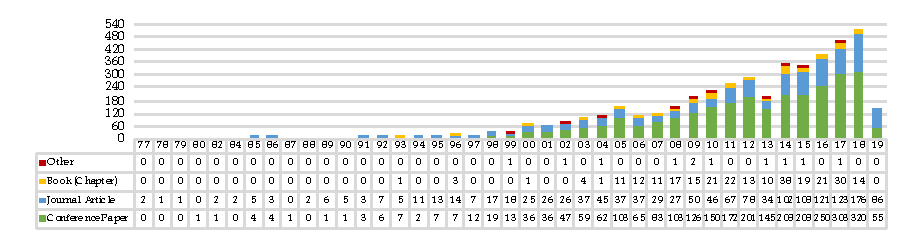
\includegraphics[width=\linewidth]{slr-years.pdf}
  \caption[Systematic mapping study search results, by years]{Search results by year and venue type.}
  \label{tse2020:fig:slr-years}
\end{figure*}

\begin{figure*}[t]
\centering
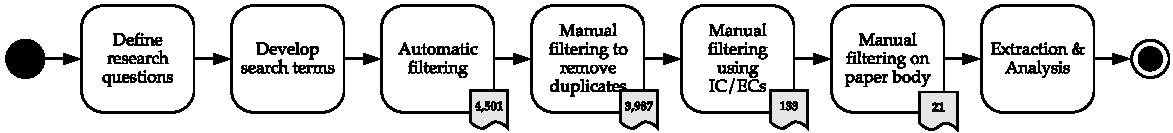
\includegraphics[width=\linewidth]{filtering.pdf}
\caption[Filtering steps used in the systematic mapping study]{A high level overview of the filtering steps from defining and executing our search query to the data extraction of our primary studies. Number of accepted papers resulting from each filtering step is shown.}
\label{tse2020:fig:filtering}
\end{figure*}
\end{landscape}}

\subsubsection{Research Questions (RQs)}

The first step in producing our \gls{sms} was to pose two RQs:
\begin{itemize}[leftmargin=\parindent]
  \item \textbf{RQ1:} What knowledge do \glsac{api} documentation studies contribute?
  \item \textbf{RQ2:} How is \glsac{api} documentation studied?
\end{itemize}
Our intent behind RQ1 was to collect as many studies provided by literature on how \glsac{api} documentation should be written using natural language (i.e., not using assistive tooling). This helped us shape and form the taxonomy provided in \cref{tse2020:sec:findings}. Secondly, RQ2's intent was to understand how the studies derive at their conclusions, thereby helping us identify gaps in literature where future studies can potentially focus.

%\begin{itemize}
%  \item RQs to help guide the \gls{sms} is:
%  \item What studies provide recommendations to improve \glsac{api} documentation? 
%  \item What is the chief methodology used to come up with these recommendations?
%  \item What is the number of methodologies and can the mapped togetjer?
%  \item Describe RQ1--3 in a systematic way
%\end{itemize}

\subsubsection{Automatic Filtering}

As done in similar \gls{se} studies~\citep{Glass:2002wa,Usman:2017hn,GAROUSI2019101}, we explored  automatic filtering of online databases. We defined which SWEBOK  knowledge areas~\citep{IEEE:1990wp} were relevant to devise a search query. Our search query was built using related knowledge areas, relevant synonyms, and the term `\glslong{se}' (for comprehensiveness) all joined with the OR operator. Due to the lack of a standard definition of an \glsac{api}, we include the terms: `\glsac{api}' and its expanded term; software library, component and framework; and lastly \gls{sdk}. These too were joined with the OR operator, appended with an AND. Lastly, the term `documentation' was appended with an AND.
Our final search string was:
% \FrameSep2pt
\begin{framed}
\noindent
\parbox{\linewidth}{
\scriptsize
( ``software design'' \textbf{OR} ``software architecture" \textbf{OR} ``software construction" \textbf{OR} ``software development" \textbf{OR} ``software maintenance" \textbf{OR} ``\gls{se} process" \textbf{OR} ``software process" \textbf{OR} ``software lifecycle" \textbf{OR} ``software methods" \textbf{OR} ``software quality" \textbf{OR} ``\gls{se} professional practice" \textbf{OR} ``\gls{se}" ) \textbf{AND} ( \glsac{api} \textbf{OR} ``application programming interface" \textbf{OR} ``software library" \textbf{OR} ``software component" \textbf{OR} ``software framework" \textbf{OR} sdk \textbf{OR} ``software development kit" ) \textbf{AND} ( documentation )
}
\end{framed}

We executed the query on all available metadata (title, abstract and keywords) in May 2019 against Web of Science\footnoteurl{http://apps.webofknowlegde.com}{23 May 2019}  (WoS), Compendex/Inspec\footnoteurl{http://www.engineeringvillage.com}{23 May 2019} (C/I) and Scopus\footnoteurl{http://www.scopus.com}{23 May 2019}. We selected three particular primary sources given their relevance in \gls{se} literature (containing the IEEE, ACM, Springer and Elsevier databases) and their ability to support advanced queries~\citep{Brereton:2007by,Kitchenham:2007dd}. A total 4,501 results\footnote{Raw results can be located at \url{http://bit.ly/2KxBLs4}.} were found, with 549 being duplicates. \Cref{tse2020:tab:search-results} displays our results in further detail (duplicates not omitted); \cref{tse2020:fig:slr-years} shows an exponential trend of \glsac{api} documentation publications produced within the last two decades. (As this search was conducted in May 2019, results taper in 2019.)

\begin{table}[tb]
  \caption[Summary of search results in API documentation knowledge]{Search results and publication types}
  \label{tse2020:tab:search-results}
  \centering
  \begin{tabular}{l|lll|l}
    \toprule
    \textbf{Publication type} &
    \textbf{WoS} &
    \textbf{C/I} &
    \textbf{Scopus} &
    \textbf{Total} \\
    \midrule
    Conference Paper & 27 & 442 & 2353 & 2822 \\
    Journal Article & 41 & 127 & 1236 & 1404\\
    Book & 23 & 17 & 224 & 264\\
    Other & 0 & 5 & 6 & 11\\
    \midrule
    \textbf{Total} & 91 & 591 & 3819 & 4501\\
    \bottomrule
  \end{tabular}
\end{table}

%\begin{itemize}
%  \item as done by Usman et al. we look at \gls{swebok} for guiding key principles in \glsac{api} development and usage. Synonyms were used as per Usman for relevant area
%  \item Lastly, we use documentation and document and *doc (e.g. Javadoc).
%  \item Insert query used: (( "software design" OR "software architecture" OR "software construction" OR "software development" OR "software maintenance" OR "\gls{se} process" OR "software process" OR "software lifecycle" OR "software methods" OR "software quality" OR "\gls{se} professional practice" OR "\gls{se}" ) AND ( \glsac{api} OR "application programming interface" OR "software library" OR "software component" OR "software framework" OR sdk OR "software development kit" ) AND ( documentation OR *docs )
%  \item What sources were used: Scopus, Compendex/Inspec (C/I) and Web of Science  (WoS) selected as they include most important \gls{se} databases IEEE Springer Elsevier and ACM. They can also handle advanced query strings. 
%  \item Queries were applied in May 2019 on all metadata (title, abstract and author keywords). 
%  \item Insert a table including number of sources.
%\end{itemize}

\subsubsection{Manual Filtering}

A follow-up manual filtering stage followed the 4,501 results obtained by automatic filtering. As described below, we applied the following inclusion criteria (IC) and exclusion criteria (EC) to each result:

\begin{enumerate}[leftmargin=2\parindent,label=\textbf{IC\arabic*}]
  \item Studies must be relevant to \glsac{api} documentation: specifically, we exclude studies that deal with improving the technical \glsac{api} usability (e.g., improved usage patterns);
  \item Studies must propose new knowledge or recommendations to document \glsacpl{api};
  \item Studies must be relevant to \gls{se} as defined in SWEBOK;
\end{enumerate}
\begin{enumerate}[leftmargin=2\parindent,label=\textbf{EC\arabic*}]
  \item Studies where full-text is not accessible through standard institutional databases; 
  \item Studies that do not propose or extend how to improve the official, natural language documentation of an \glsac{api};
  \item Studies proposing a third-party tool to enhance existing documentation or generate new documentation using data mining (i.e., not proposing strategies to improve official documentation);
  \item Studies not written in English;
  \item Studies not peer-reviewed.
\end{enumerate}
\smallskip

Each of these ICs and ECs were applied to every paper  after exporting all  metadata of our results to a spreadsheet. The first author then curated the publications using the following revision process.

Firstly, we read the publication source---to rapidly omit non-\gls{se} papers---as well as the author keywords, title, and abstract of all 4,501 studies. As some studies were duplicated between our three primary sources, we needed to remove any repetitions. We sorted and reviewed any duplicate DOIs and fuzzy-matched all very similar titles (i.e., changes due to punctuation between primary sources), thereby retaining only one copy of the paper from a single database. Similarly, as there was no limit do our date ranges, some studies were republished in various venues (i.e., same title but different DOIs). These were also removed using fuzzy-matching on the title, and the first instance of the paper's publication was retained. This second phase resulted in 3,987 papers.

Secondly, we applied our inclusion and exclusion criteria to each of the 3,987 papers by reading the abstract. Where there was any doubt in applying the criteria to the abstract alone, we automatically shortlisted the study. We rejected 427 studies that were unrelated to \gls{se}, 3,235 were not directly related to documenting \glsacpl{api} (e.g., to enhance coding techniques that improve the overall developer usability of the \glsac{api}), 182 proposed new tools to enhance \glsac{api} documentation or used machine learning to mine developer's discussion of \glsacpl{api}, and 10 were not in English. This resulted in 133 studies being shortlisted to the final phase.

Thirdly, we re-evaluated each shortlisted paper by re-reading the abstract, the introduction and conclusion. We removed a further 64 studies that were on \glsac{api} usability or non \glsac{api}-related  documentation (i.e., code commenting). At this stage, we decided to refine our exclusion criteria to better match the research goals of this study by including the word `natural language' documentation in EC2. This removed studies where the focus was to improve technical documentation of \glsacpl{api} such as data types and communication schemas. Additionally, we removed 26 studies as they were related to introducing new tools (EC3), 3 were focused on tools to mine \glsac{api} documentation, 7 studies where no recommendations were provided, 2 further duplicate studies, and a further 10 studies where the full text was not available, not peer reviewed or in English. Books are commonly not peer-reviewed (EC5), however no books were shortlisted within these results. This final stage resulted in 21 primary studies for further analysis, and the mapping of primary study identifiers to references S1--21 can be found in \cref{tse2020:sec:primary-sources}.

As a final phase, we conducted reliability analysis of our shortlisting method. We conducted intra-rater reliability of our 133 shortlisted papers using the test-retest approach suggested by~\citet{Kitchenham:2007dd}. We re-evaluated a random sample of 10\% of the 133 shortlisted papers a week after initial studies were shortlisted. This resulted in \textit{substantial agreement}~\citep{Landis:1977kv}, measured using Cohen's kappa ($\kappa=0.7547$).
%THREAT To VALIDITY: While~\citep{Kitchenham} describes that single researcher (e.g., PhD student) should discuss externally, wasn't possible. Does suggest the test-retest method which was chosen. No inter-rater reliability is yet determined at this stage but open for future work.

\subsubsection{Data Extraction \& Systematic Mapping}
\label{tse2020:sec:data-extraction}

Of the 21 primary studies, we conducted abstract key-wording adhering to~\citeauthor{Petersen:2008td}'s guidelines~\citep{Petersen:2008td} to develop a classification scheme.
An initial set of keywords were applied for each paper in terms of their methodologies and research approaches (RQ2), based on an existing classification schema used in the requirements engineering field by~\citet{Wieringa:2006vd}. These are: \textit{evaluation papers}, which evaluates existing techniques in-practice; \textit{validation papers}, which investigates proposed techniques not yet implemented in-practice; \textit{experience papers}, which do investigate or evaluate either proposed or existing techniques, but presents insightful experiences of authors that warrant communication to other practitioners; and \textit{philosophical papers}, which presents new conceptual frameworks that describes a language by which we can describes our observations of existing or new techniques, thereby implying a new viewpoint for understanding phenomena.

After all primary studies had been assigned keywords, we noticed that all papers used field study techniques, and thus we consolidated these keywords using~\citeauthor{Singer:2007tu}'s framework of \gls{se} field study techniques~\citep{Singer:2007tu}.~\citeauthor{Singer:2007tu} captures both study techniques \textit{and} methods to collect data within the one framework, namely: \textit{direct techniques}, including brainstorming and focus groups, interviews and questionnaires, conceptual modelling, work diaries, think-aloud sessions, shadowing and observation, participant observation; \textit{indirect techniques}, including instrumenting systems, fly-on-the-wall; and \textit{independent techniques}, including analysis of work databases, tool use logs, documentation analysis, and static and dynamic analysis. 

\Cref{tse2020:tab:extraction} describes our data extraction form, which was used to collect relevant data from each paper. \Cref{tse2020:fig:sms} presents our systematic mapping, where each study is mapped to one (or more, if applicable) of methodologies plotted against~\citeauthor{Wieringa:2006vd}'s research approaches. We find that a majority of these studies survey developers using direct techniques (i.e., interviews and questionnaires) and some performing structured documentation analysis. Few studies report recent experiences, with the majority of \glsac{api} documentation knowledge being evaluation research, and some validation studies. There are few experience papers describing anecdotal evidence of \glsac{api} documentation knowledge, and almost no philosophical papers that describe new conceptual ways at approaching \glsac{api} documentation as a large majority of existing work either evaluates existing (in-practice) strategies or validates the effectiveness of new strategies.

\begin{table}[tb]
  \caption[Data extraction in API documentation knowledge study]{Data extraction form}
  \label{tse2020:tab:extraction}
  \centering
  \begin{tabular}{l|p{0.6\linewidth}}
    \toprule
    \textbf{Data item(s)} &
    \textbf{Description}
    \\
    \midrule
    Citation metadata & Title, author(s), years, publication venue, publication type \\
    Key recommendation(s) & As per IC2, the study must propose at least one recommendation on what should be captured in \glsac{api} documentation \\
    Evaluation method & Did the authors evaluate their recommendations? If so, how? \\
    Primary technique & The primary technique used to devise the recommendation(s) \\ 
    Secondary technique & As above, if a second study was conducted \\
    Tertiary technique & As above, if a third study was conducted \\
    Research type & The research type employed in the study as defined by~\citeauthor{Wieringa:2006vd}'s taxonomy \\
    \bottomrule
  \end{tabular}
\end{table}

\subsection{Development of the Taxonomy}
\label{tse2020:sec:method:taxonomy-development}


A majority of taxonomies produced in \gls{se} studies are often made extemporaneously~\citep{Usman:2017hn}. For this reason, we decided to proceed with a systematic approach to develop our taxonomy using the guidelines provided by~\citet{Usman:2017hn}, which are extended from lessons learned in more mature domains. In this subsection, we outline the 4 phases and 13 steps taken to develop our taxonomy based on~\citeauthor{Usman:2017hn}'s technique.~\citeauthor{Usman:2017hn}'s final \textit{validation} phase is largely detailed within \cref{tse2020:sec:validation} after we present our taxonomy in \cref{tse2020:sec:findings}.

\subsubsection{Planning phase} The preliminary phase involves answering the following:

\begin{figure}[t!]
  \centering
  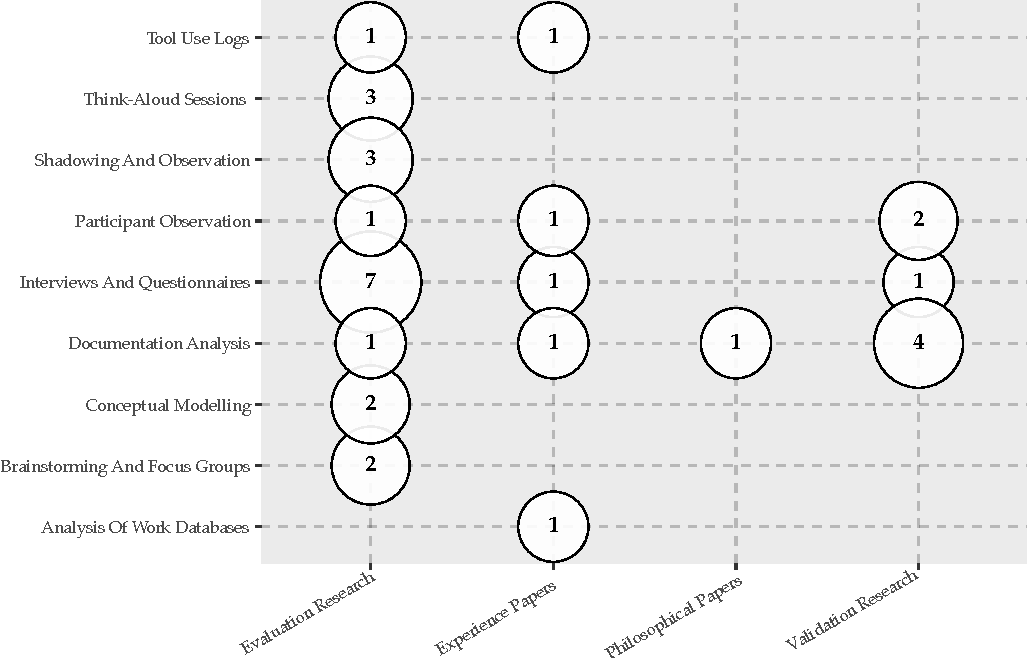
\includegraphics[width=.8\linewidth]{sms}
  \caption[A systematic map of API documentation knowledge studies]{Systematic map: field study technique vs research type}
  \label{tse2020:fig:sms}
\end{figure}

\begin{enumerate}[label=\textbf{(\arabic*)}]
  \item \textit{define the \gls{se} knowledge area}: The \gls{se} knowledge area, as defined by the SWEBOK, is software construction;
  \item \textit{define the objective}: The main objective of the proposed taxonomy is to define a set of categories that enables to classify different facets of natural-language \glsac{api} \textit{documentation} knowledge (not \glsac{api} \textit{usability} knowledge) as reported in existing literature;
  \item \textit{define the subject matter}: The subject matter of our proposed taxonomy is  documentation artefacts of \glsacpl{api};
  \item \textit{define the classification structure}: The classification structure of our  proposed taxonomy is \textit{hierarchical};
  \item \textit{define the classification procedure}: The procedure used to classify the documentation artefacts is qualitative; 
  \item \textit{define the data sources}: The basis of the taxonomy is derived from field study techniques (see \cref{tse2020:sec:data-extraction}).
\end{enumerate}

\subsubsection{Identification and extraction phase} The second phase of the taxonomy development involves \textbf{(7)}~\textit{extracting all terms and concepts} from relevant literature, which we have achieved from our \gls{sms}. These terms are then consolidated by \textbf{(8)}~\textit{performing terminology control}, as some terms may refer to different concepts and vice-versa.

\subsubsection{Design phase} The design phase identified the core dimensions and categories within the extracted data items. The first step is to \textbf{(9)}~\textit{identify and define taxonomy dimensions}; for this study we utilised a bottom-up approach to identify each dimension, i.e., extracting the categories first and then nominating which dimensions these categories fit into using an iterative approach. As we used a bottom-up approach, step (9) also encompassed the second stage of the design phase, which is to \textbf{(10)}~\textit{identify and describe the categories} of each dimension. Thirdly, we \textbf{(11)}~\textit{identify and describe relationships} between dimensions and categories, which can be skipped if the relationships are too close together, as is the case of our grouping technique which allows for new dimensions and categories to be added. The last step in this phase is to \textbf{(12)}~\textit{define guidelines for using and updating the taxonomy}. The taxonomy is as simple as a checklist that can be heuristically applied to an \glsac{api} document, and each dimension is malleable and covers a broad spectrum of artefacts; while we do not anticipate any further dimensions to be added, new categories can easily be fitted into one of the dimensions (see \cref{tse2020:sec:conclusions}). We provide guidelines for use in our application of the taxonomy against \glspl{cvs} within \cref{tse2020:sec:findings,tse2020:sec:tax-analysis}.

\subsubsection{Validation phase} In the final phase of taxonomy development, taxonomy designers must \textbf{(13)}~\textit{validate the taxonomy} to assess its usefulness.~\citet{Usman:2017hn} describe three approaches to validate taxonomies: (i) orthogonal demonstration, in which the taxonomy's orthogonality is demonstrated against the dimensions and categories, (ii) benchmarking the taxonomy against similar classification schemes, or (iii) utility demonstration by applying the taxonomy heuristically against subject-matter examples. In our study, we adopt utility demonstration by use of a survey and heuristic application of the taxonomy against real-world case-studies (i.e., within the domain of \glspl{cvs}). This is is discussed in greater detail within \cref{tse2020:sec:validation}.


\section{\glsac{api} Documentation Knowledge Taxonomy}
\label{tse2020:sec:findings}

\begin{figure}[p]
\centering
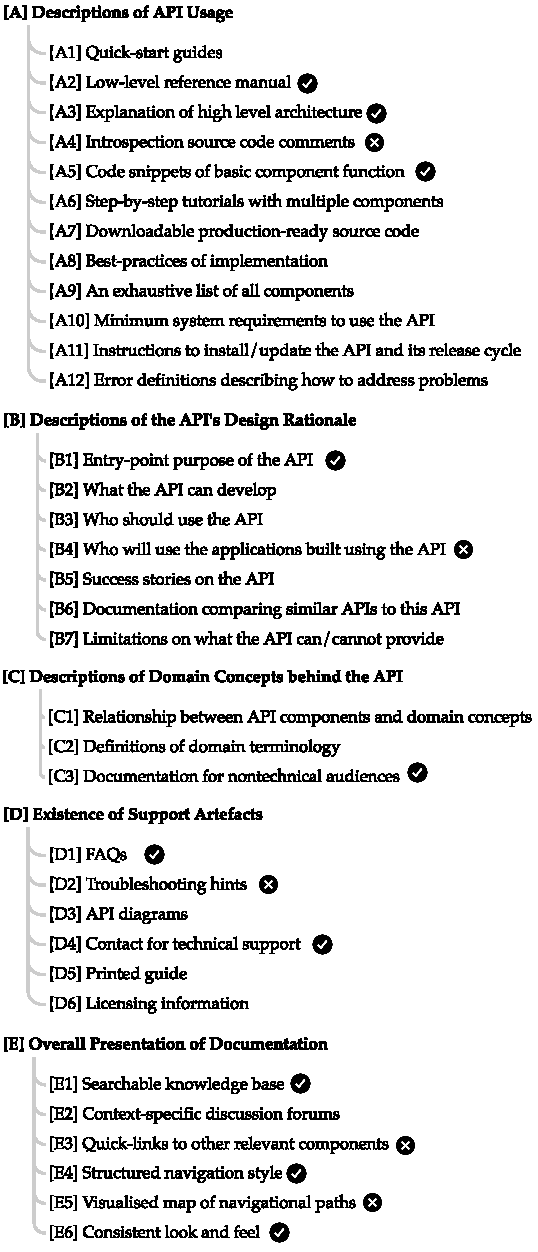
\includegraphics[width=.85\linewidth]{taxonomy}
\caption[Our proposed API documentation knowledge taxonomy]{Our proposed taxonomy on what artefacts should be documented in a complete \glsac{api} document.} %Underlined are key artefacts of interest. The top five ILS knowledge artefacts, highlighting what \textit{literature} anticipates is most useful, is indicated using the book symbol. The top five IPS knowledge artefacts, highlighting what \textit{practitioners} say is most useful, is indicated using with the computer symbol. The five agreements between ILS and IPS values (within a standard deviation of 0.15) are indicated with handshake symbols, where VH =~Very Helpful, SH~=~Slightly Helpful, NH~=~Not Helpful. Checkmarks indicate that all three \glspl{cvs} assessed include the category, while crosses indicate that all three \glspl{cvs} do not include the category.}
\label{tse2020:fig:taxonomy}
\end{figure}

Our taxonomy consists of five dimensions (labelled A--E). We expand these five dimensions into 34 categories (sub-dimensions). Each dimension respectively covers:
\begin{itemize}
  \item \textbf{[A]~\dima{}} on \textit{how} to use the \glsac{api} for the developer's intended use case;
  \item \textbf{[B]~\dimb{}} on \textit{when} the developer should choose this \glsac{api} for a particular use case;
  \item \textbf{[C]~\dimc{}} of the domain behind the \glsac{api} to understand \textit{why} this \glsac{api} should be chosen for this domain;
  \item \textbf{[D]~\dimd{}} that describe \textit{what} additional documentation the \glsac{api} provides; and
  \item \textbf{[E]~\dime{}} to help organise the \textit{visualisation} of the above information.
\end{itemize}
Further descriptions of the categories encompassing each dimension are given within \cref{tse2020:fig:taxonomy,tse2020:tab:taxonomy}, coded as [$Xi$], where $i$ is the category identifier within a dimension, $X$, where $X~\in~\{ A, B, C, D, E \}$.

\Cref{tse2020:tab:taxonomy} shows which of the primary sources (S1--21) provide the recommendation described as well as an `in-literature score' (ILS). This score is a weighting calculated as a percentage of the number of primary studies that make the recommendation divided by the total of primary studies, and indicates the overall level of agreement that academic sources suggest these documentation artefacts. This score is contrasted to the `in-practice score' (IPS) which indicates the overall level of agreement that \textit{practitioners} think such documentation artefacts are needed. Further details about the ILS and IPS values, how they were calculated and analysed for each category, and a rigorous contrast between the two are provided \cref{tse2020:sec:validation:survey:eval,tse2020:sec:tax-analysis:ils,tse2020:sec:tax-analysis:ips,tse2020:sec:tax-analysis:ils-vs-ips}. For comparative purposes, we illustrate a colour scale (from red to green) to indicate the relevancy weight between ILS and IPS values in \cref{tse2020:tab:taxonomy}: for example, while quick-start guides \dimcat{A1} are few referenced in academic sources at 14\%, they are generally well-desired by practitioners 88\% agreement. We then provide three columns that assesses the presence of these documentation artefacts against three popular \glspl{cvs}: Google Cloud Vision, AWS's Rekognition, and Azure Cloud Vision (abbreviated to GCV, AWS and ACV). A fully shaded circle~(\circlepresent{}) indicates that the documentation artefact was clearly found in the service, while a half-shaded circle~(\circlepartialpresent{}) indicates that the artefact was only partially present. An outlined circle~(\circlenotpresent{}) indicates that the service lacks the indicated documentation artefact within our taxonomy. This empirical assessment is further detailed in \cref{tse2020:sec:tax-analysis:cvs-improvement}, which outlines concrete areas in the respective services' documentation where improvements could be made, as well as hyperlinks to the documentation where relevant. 

\Cref{tse2020:fig:taxonomy} illustrates these findings, with underlines indicating key artefacts and various iconography to indicate specific results. The computer icon~(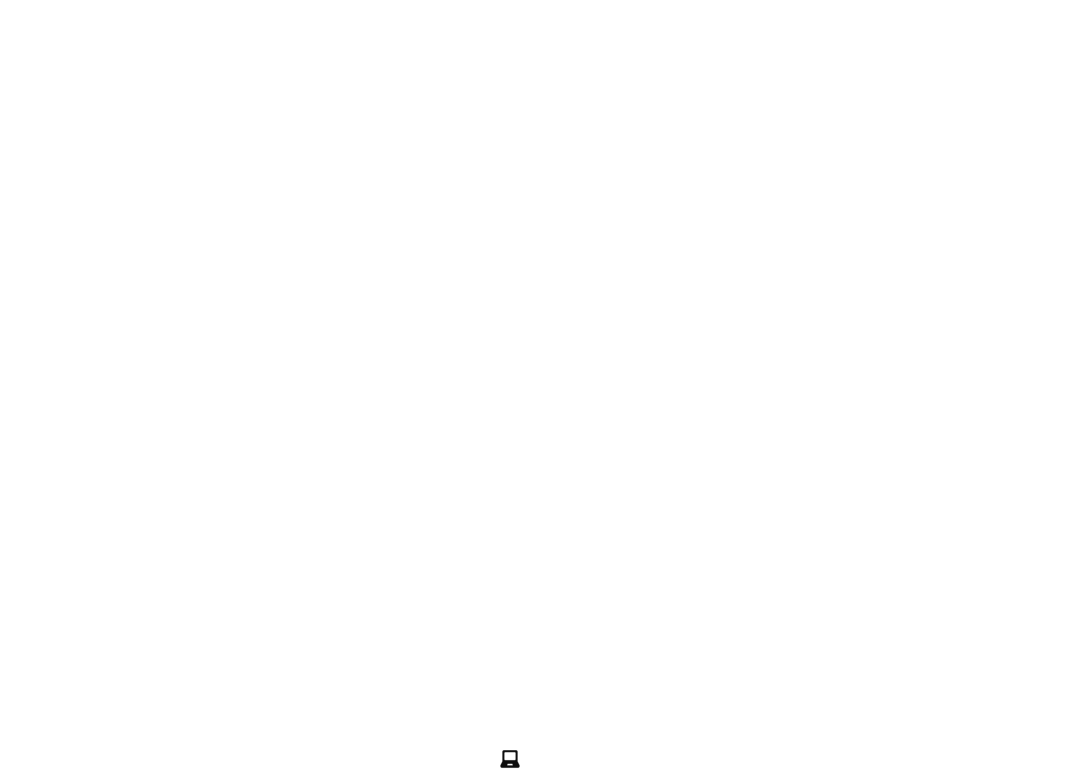
\includegraphics{computer}) includes a ranking from 1--5 of the top five most recommended artefacts according to developers, as calculated from their relevant IPS scores. Conversely, the book icon~(\,
\includegraphics{book}\,) indicates the rankings of the top five most recommended artefacts according to literature. For example, while literature suggests the most useful documentation artefact are \glsac{api} usage description code snippets \dimcat{A5}, in-practice, we find that developers prefer design rationale on what the limitations of \glsac{api} are \dimcat{B7} with code snippets coming in second place. Where there is strong agreement between developers and literature (within a standard deviation of 0.15) we use the handshake icon~(\,
\includegraphics{handshake}\,) and list whether both agree if the category is Very Helpful~(VH), Slightly Helpful~(SH) or Not Helpful~(NH). Further details on this explanation are provided in \cref{tse2020:sec:tax-analysis:ils-vs-ips}. Lastly, we provide iconography for the presence~(\faCheckCircle) or non-presence~(\faTimesCircle) of these   artefacts in \textit{all three} \glspl{cvs} assessed, per \cref{tse2020:sec:tax-analysis:ips}.


\section{Validating our Taxonomy}
\label{tse2020:sec:validation}

\subsection{Survey Study}
\label{tse2020:sec:validation:survey}

\subsubsection{Designing the Survey}

We followed the guidelines by~\citet{Kitchenham:2007ux} on conducting personal opinion surveys in \gls{se} to validate our survey. In developing our survey instrument, we  shaped questions around each of our 5 dimensions and 34 categories. To achieve this, we used~\citeauthor{Brooke:1996ua}'s \gls{sus}~\citep{Brooke:1996ua} as inspiration and re-shaped the 34 categories around a question. Each dimension was marked a numeric question (3--7), and alphabetic sub-questions were marked for each sub-dimension or category.

 We used closed questioning where respondents could choose an answer on a 5-point Likert-scale (1=\textit{strongly disagree}, 2=\textit{somewhat disagree}, 3=\textit{neither agree nor disagree}, 4=\textit{slightly agree} and 5=\textit{strongly agree}).  Like~\citeauthor{Brooke:1996ua}'s study, each question alternated in positive and negative sentiment. Half of our questions were written where a likely common response would be in strong agreement and vice-versa for the other half, such that participants would have to ``read each statement and make an effort to think whether they would agree or disagree with it''~\citep{Brooke:1996ua}. For example, the question regarding \dimcat{B7} on \glsac{api} limitations was framed as: ``\textit{I believe it is important to know about what the limitations are on what the \glsac{api} can and cannot provide}'' (Q4g), whereas the question regarding \dimcat{C1} on domain concepts of the \glsac{api} was framed as: ``\textit{I wouldn't read through theory about the API's domain that relates theoretical concepts to \glsac{api} components and how both work together}'' (Q5a). 
 
 In addition, the remaining eight questions asked demographical information. An extra open question asked for further comments. The full survey is provided in \cref{tse2020:sec:survey}.

\subsubsection{Evaluating the Survey}
\label{tse2020:sec:validation:survey:eval}

After the first pass at designing questions was completed, we evaluated our survey on three researchers within our research group for general feedback. This resulted in minor changes, such as slight re-wording of questions, clarifying the difference between web services and web \glsacpl{api}, and providing specific questions with examples (some with images). For example, the question regarding \dimcat{A9} on an exhaustive list of all major components in the \glsac{api} was framed as ``\textit{I believe an exhaustive list of all major components in the \glsac{api} without excessive detail would be useful when learning an \glsac{api}}'' (Q3i) with the example ``\textit{e.g., a \gls{cv} web \glsac{api} might list object detection, object localisation, facial recognition, and facial comparison as its 4 components}''.

After this, we conducted reliability analysis using a test-retest approach on three developers within our group seven weeks apart.  This was calculated using the \texttt{irr} computational R package~\citep{Gamer:tj} (as suggested in~\citep{Hallgren:2012kt}) and  resulted in an average intra-class correlation of 0.63 which indicates a good overall index of agreement~\citep{cicchetti1994guidelines}.

\subsubsection{Recruiting Participants}

Our target population for the study was application software developers with varying degrees of experience (including those who and who have not used \glspl{cvs} or related tools before) and varying understanding of fundamental machine learning concepts. We began by recruiting software developers within our research group using a group-wide message sent on our internal messaging system. Of the 44 developers in our group's engineering cohort, 22 responses were returned, indicating an internal response rate of 50\%.

For external participant recruiting, we shared the survey on social media platforms and online-discussion forums relevant to software development. We adopted a non-probabilistic snowballing sampling where the participants, at the end of the survey, were encouraged to share the survey link to others using \textit{AddThis}\footnote{\url{https://www.addthis.com} last accessed 7 January 2020}. This resulted in 43 additional visits to the survey. Additionally, snowballing sampling was encouraged within members of our research group who shared the survey with an additional 21 participants. However, while there were a total of 86 respondents, only 51 finished the survey, leaving 35 participants with partially completed responses. Our final response rate was therefore 59\%, which is very close to median response rates of 60\%~\citep{Baruch:1999vf} in information systems and 5\% in \gls{se}~\citep{Singer:2007tu}.

\subsubsection{Analysing Response Data}
\label{tse2020:sec:validation:survey:analysis}

To analyse our response data, we used an adapted version of the \gls{sus} method to produce a score for each question's 5-point response. As per~\citeauthor{Brooke:1996ua}'s methodology, we mapped the responses from their ordinal scale of 1--5 to 0--4, and subtracted that value by 1 for positive questions and subtracted the value from 5 for the negative questions~\citep{Brooke:1996ua}. Unlike~\citeauthor{Brooke:1996ua}'s method, we averaged each response for every question and divided by four (i.e, now a 4-point scale) to obtain scores for each category. This is presented in \cref{tse2020:tab:taxonomy} under the `in-practice score' (IPS) for each category.

Demographics for our survey were consistent in terms of the experience levels of developers who responded. Most were professional programmers with 75\% reporting between 1--10 years of work experience. A majority of our respondents (33\%) reported to be in mid-tier roles. Most worked in either consulting or information technology services, reported at 17\% for both.

\subsection{Empirical application of the taxonomy against Computer Vision Services}

Once our taxonomy had been developed, we performed an empirical application against three \glspl{cvs}: Google Cloud Vision~\citepweb{GoogleCloud:Home}, Amazon Rekognition~\citepweb{AWS:Home} and Azure Computer Vision~\citepweb{Azure:Home}. Our selection criteria in choosing these particular services to analyse is based on the prominence of the service providers in industry and the ubiquity of their cloud platforms (Google Cloud, Amazon Web Services, and Microsoft Azure) in addition to being the top three adopted vendors used for cloud-based enterprise applications~\citep{RightScaleInc:2018kJ}. In addition, we had conducted extensive investigation into the services' non-deterministic runtime behaviour and evolution profile in prior work~\citep{Cummaudo:2019icsme} and have also identified developers' complaints about their incomplete documentation in a prior mining study on Stack Overflow~\citep{Cummaudo:2020icse}.

We began with an exploratory analysis of the presence of each dimension and its categories. \Cref{tse2020:tab:docsources} displays all sources of documentation used; although we initially started on the respective services homepages~\citepweb{GoogleCloud:Home,AWS:Home,Azure:Home}, this search was expanded to other webpages hyperlinked. For each category, we listed the documentation's presence as either fully present, partially present or not present at all. This is shown in \cref{tse2020:tab:taxonomy} with the indication of (half-)filled circles or circle outlines for Google Cloud Vision (abbreviated to GCV), Amazon Rekognition (abbreviated to AWS), and Azure Computer Vision (abbreviated to ACV). Notes were taken for each webpage justifying the presence, and exact sources of documentation were listed when (partially) present. PDFs of each webpage were downloaded between 14--18 March 2019 for analysis.

Once our analysis was completed and results from the survey finalised, we then calculated \textit{weighted} ILS and IPS values for each dimension's category. This was done by multiplying the ILS and IPS values for each category (listed in \cref{tse2020:tab:taxonomy}) by either 0, 0.5 or 1 for categories not present, partially present, or present (respectively) in each service. The `maximum' ILS and IPS values indicate the highest possible score a service can be ranked as though \textit{all} categories are present. \Cref{tse2020:tab:weighted-ils,tse2020:tab:weighted-ips} show the sum of weights for each category in its respective dimension, in addition to the maximum possible score. Again, we use the same abbreviations for each service as per \cref{tse2020:tab:taxonomy}. The scores are normalised into percentages for comparative purposes as a ratio of the score over all dimensions for a particular service to the maximum possible score. For comparative purposes, these are illustrated in \cref{tse2020:fig:scorecompare}.

\begin{table}[tbh]
  \centering
  \caption[Weighted ILS Scoring]{Weighted ILS Scoring.}%GCV = Google Cloud Vision, AWS = Amazon Rekognition, ACV = Azure Computer Vision.
  \label{tse2020:tab:weighted-ils}
  \tablefit{
  \begin{tabular}{l|ccc|c}
    \toprule
    \textbf{Dimension} & \textbf{GCV} & \textbf{AWS} & \textbf{ACV} & \textbf{Max}
    \\
    \midrule
    \relax[A] Usage Description &2.64 (60\%)&3.10 (71\%)&3.02 (69\%)&4.38\\
    \relax[B] Design Rationale&0.79 (55\%)&0.95 (67\%)&0.95 (67\%)&1.43\\
    \relax[C] Domain Concepts&0.33 (54\%)&0.14 (23\%)&0.43 (69\%)&0.62\\
    \relax[D] Support Artefacts&0.24 (31\%)&0.52 (69\%)&0.50 (66\%)&0.76\\
    \relax[E] Documentation Presentation&1.05 (79\%)&1.05 (79\%)&0.98 (73\%)&1.33\\
    \midrule
    Total&5.05 (59\%)&5.76 (68\%)&5.88 (69\%)&8.52\\
    \bottomrule
  \end{tabular}}
  \bigskip
  \caption[Weighted IPS Scoring]{Weighted IPS Scoring.}
  \label{tse2020:tab:weighted-ips}
  \footnotesize
  \tablefit{
  \begin{tabular}{l|ccc|c}
    \toprule
    \textbf{Dimension} & \textbf{GCV} & \textbf{AWS} & \textbf{ACV} & \textbf{Max}
    \\
    \midrule
    \relax[A] Usage Description &4.84 (57\%)&5.26 (62\%)&5.62 (66\%)&8.48\\
    \relax[B] Design Rationale&1.78 (43\%)&2.51 (61\%)&2.51 (61\%)&4.13\\
    \relax[C] Domain Concepts&0.92 (51\%)&0.55 (31\%)&1.43 (80\%)&1.80\\
    \relax[D] Support Artefacts&0.96 (28\%)&1.80 (53\%)&1.85 (55\%)&3.36\\
    \relax[E] Documentation Presentation&2.66 (70\%)&2.66 (70\%)&2.38 (63\%)&3.79\\
    \midrule
    Total&11.17 (52\%)&12.79 (59\%)&13.79 (64\%)&21.56\\
    \bottomrule
  \end{tabular}}
\end{table}

\section{Taxonomy Analysis}
\label{tse2020:sec:tax-analysis}

In this section, we analyse investigating the taxonomy from two perspectives. Firstly, we describe the ILS values, being an interpretation of the number of papers that conclude the recommendations in each category and dimension, and the weighted ILS scores, being an application of the taxonomy specifically to \glspl{cvs}. Secondly, we look at the results from our survey and their respective IPS values, being an interpretation of how well developers agree with these recommendations, and the weighted IPS scores, being the application of how application developers would agree with the documentation of the \glspl{cvs}. We then contrast the difference between what literature recommends and how well developers agree with these recommendations.

\subsection{In-Literature Scores for Taxonomy Categories}
\label{tse2020:sec:tax-analysis:ils}

ILS values indicate the proportion of papers that recommend categories within our taxonomy of all 21 studies. The most highly recommended categories from our \gls{sms} fall under the \dima{} dimension. The majority (0.71) of studies advocate for code snippets as a necessary piece in the \glsac{api} documentation puzzle \dimcat{A5}. While code snippets generally only reflect small portions of \glsac{api} functionality (limited to 15--30 LoC), this is complimented by step-by-step tutorials (0.57) that tie in multiple (disparate) components of \glsac{api} functionality, generally with some form of screenshots, demonstrating the development of a non-trivial application using the \glsac{api} step-by-step \dimcat{A6}. The third highest category scored was also under the \dima{} dimension, being low-level reference documentation at 0.52 \dimcat{A2}. These three categories were the only categories to be scored as majority categories (i.e., their scores were above 0.50).
The fourth and fifth highest scores are an entry-level purpose/overview of the \glsac{api} (0.48) that gives a brief motivation as to why a developer should choose a particular \glsac{api} over another \dimcat{B1} and consistency in the look and feel of the documentation throughout all of the API's official documentation (0.43)~\dimcat{E6}.

\subsection{In-Practice Scores for Taxonomy Categories}
\label{tse2020:sec:tax-analysis:ips}

IPS values indicate the extent to which developers `agree' with the statements made in our survey, as calculated using the \gls{sus} technique~\citep{Brooke:1996ua}. These values are generally greater than the ILS values, since they are ranked by all survey participants and are not a ratio of the 21 primary studies. Unlike ILS scores, 28 categories scored above 0.50. The highest dimension corroborates that of the ILS scores; within the top five ranked ILS scores, \dima{} categories feature four times. However, developers generally find limitations on what the \glsacpl{api} can and cannot provide the most useful, at 0.94, which falls under the \dimb{} dimension \dimcat{B7}. Following this, the code-snippets \dimcat{A5} is highly ranked (as per the ILS values) with developers agreeing that code-snippets should be included in most \glsac{api} documentation. Quick-start guides \dimcat{A1} are the next most-useful category that developers advocate for, reported at 0.88. Following this, the instructions on how to install the \glsac{api} or begin using the \glsac{api}, its release cycle, and frequently it is updated \dimcat{A11} is also important, ranking fourth at 0.86. Lastly, error definitions describing how developers can address problems \dimcat{A12} were scored at 0.84.


\subsection{Contrasting In-Literature to In-Practice Scores}
\label{tse2020:sec:tax-analysis:ils-vs-ips}

\begin{figure*}[t]
  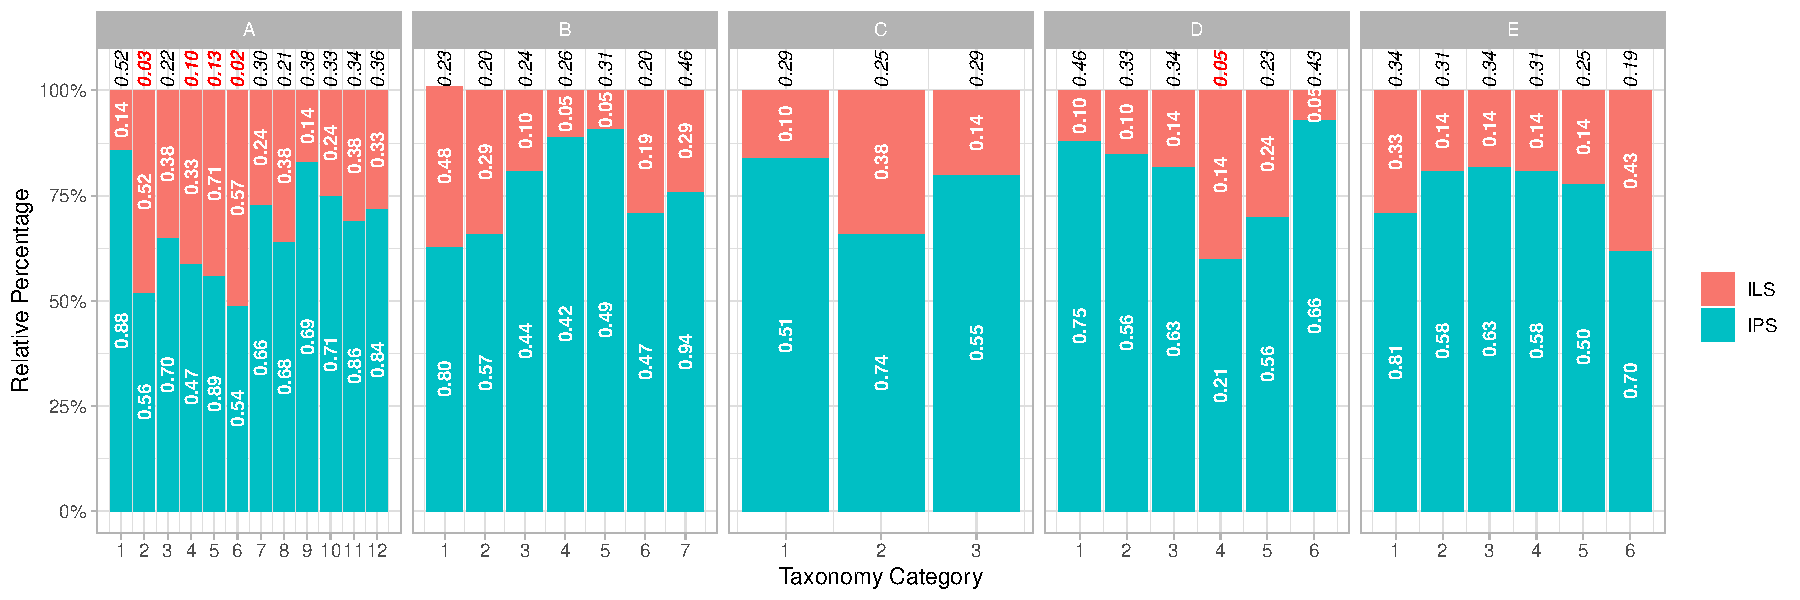
\includegraphics[width=\linewidth]{ils-vs-ips3}
  \caption[Comparison of ILS and IPS values]{Comparison of ILS and IPS values for each category (grouped by dimensions) presented as a relative percentage.}
  \label{tse2020:fig:ils-vs-ips}
\end{figure*}

\Cref{tse2020:fig:ils-vs-ips} highlights the relative percentage of each ILS and IPS value for all subcategories, thereby indicating the relative agreement between the two. In this graph, an ILS and/or IPS core approaching a relative percentage of 50\% indicates equal agreement whereby both developer's and literary references share a similar distribution of recommendation agreement. Italicised labels above each column indicates the standard deviation between the ILS and IPS values, where red labels indicated a standard deviation less than 0.15 (i.e., developers and literature agree to the values to a similar extent).

\begin{table}
  \centering
  \caption[Labels assigned to ILS and IPS values]{Labels assigned to ILS and IPS values.}
  \label{tse2020:tab:labels-for-ils-ips}
  \begin{tabular}{c|cc}
    \toprule
    \textbf{Description} & \textbf{Lower Score Bound} & \textbf{Upper Score Bound}\\
    \midrule
    \textit{Not Helpful} & 0.00 & 0.24\\
    \textit{Slightly Unhelpful} & 0.25 & 0.49 \\
    \textit{Slightly Helpful} & 0.50 & 0.74 \\
    \textit{Very Helpful} & 0.75 & 1.00\\
    \bottomrule
  \end{tabular}
\end{table}

Where the standard deviation between ILS and IPS values is less than 0.015 (as indicated by red labels above each column in \cref{tse2020:fig:ils-vs-ips}), then there is strong alignment between both scores. However, of all 34 categories, only five cases of this occur.
Developers agree to the academic works that make the recommendations \textit{to the same relative proportion} as per the labels assigned in \cref{tse2020:tab:labels-for-ils-ips}:

\begin{itemize}
  \item Having email addresses or phone numbers listed within an \glsac{api} is generally not helpful at all \dimcat{D4},
  \item Introspecting the source code comments of an \glsac{api} is only somewhat helpful \dimcat{A4},
  \item Low-level reference documentation with all objects and methods (etc.) documented is slightly helpful \dimcat{A2},
  \item Following step-by-step tutorials are also slightly helpful \dimcat{A6},
  \item Code snippets are the most helpful \dimcat{A5}.
\end{itemize}

The remaining categories in the dimension do not share strong association between both developer opinions and the number of papers producing recommendations. Due to the disparity between these ILS and IPS values, we do not report on their utility.

\subsection{Triangulating ILS and IPS with Computer Vision}

\begin{figure}[tbh]
  \centering
  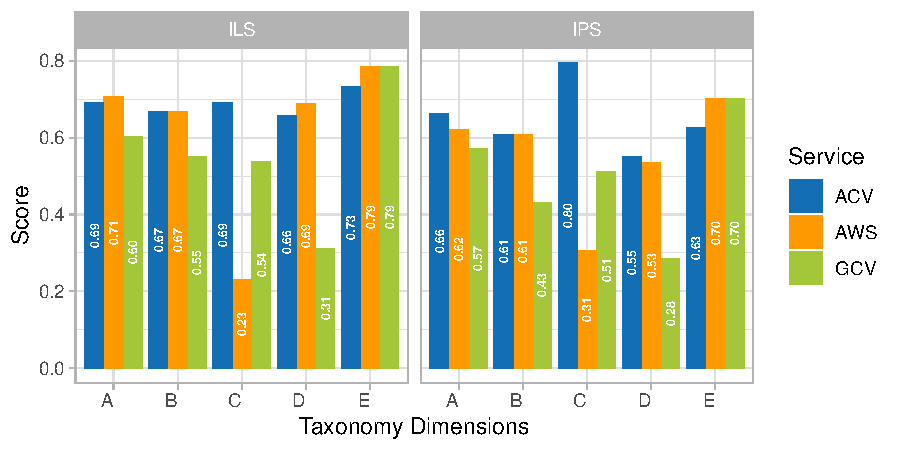
\includegraphics[width=\linewidth]{scores2}
  \caption[Comparison of ILS and IPS values]{Comparison of the weighted ILS and IPS values for the three \glspl{cvs} assessed.}
  \label{tse2020:fig:scorecompare}
\end{figure}

When applied in the context of \glspl{cvs}, we see that Azure Computer Vision (ACV) and Amazon Rekognition (AWS) are better documented than Google Cloud Vision (GCV), particularly in \dimb{} and \dima{}. \Cref{tse2020:fig:scorecompare} highlights that Azure Computer Vision is especially well documented in \dimc{} when measured using the weighted ILS and has the highest score of all services and dimensions. It is evident that Google Cloud Vision needs improved \dimb{} documentation and further \dimd{} would be helpful. Generally speaking, Google Cloud Vision is less `complete' than other services, except in \dimc{} documentation and its \dime{}.

In the context of \glspl{cvs}, IPS values share a similar distribution to ILS values. Notably, in-practice, it seems developers prefer the documentation of Amazon Rekognition compared to the the in-literature weighted scoring of Azure Computer Vision (\cref{tse2020:fig:scorecompare}). Except in the case of documenting \dimc{}, Amazon Rekognition scores slightly higher than Azure Computer Vision except for the \dimb{} documentation where it is equal. Similar to the ILS scoring, Google Computer Vision has low  compliance to the recommendations proposed, except in its \dime{}.

\subsection{Areas of Improvement for CVS Documentation}
\label{tse2020:sec:tax-analysis:cvs-improvement}

Triangulating the taxonomy developed from literary sources, the developer survey on this taxonomy to understand its efficacy in-practice, and applying the taxonomy to the \gls{cvs} domain, we are able to assess the key areas of improvement in this domain.

For this assessment, we select the ILS or IPS values for categories that are considered either somewhat or very helpful (i.e., a score greater than 0.50). We then match these against categories that are found to be partially or not present within each service. In total, we found 12 categories where improvements can be made across all dimensions except \dime{}, detailed below .

\subsubsection[Dimension A Issues]{Issues regarding \dima{}}

\paragraph{Quick-start guides \dimcat{A1}:} 
Quick-start guides should provide a short tutorial that allows programmers to pick up the basics of an \glsac{api} in a programming language of their choice. For the services assessed, each offer various client \glspl{sdk} (e.g., as Java or Python client libraries). Google Cloud Vision and Azure Computer Vision offer quick-start guides~\citepweb{Quicksta92:online,Quicksta70:online} in which sets of articles target various \glspl{sdk} or are client-agnostic with code snippets that can be changed to the client language/\gls{sdk} of the developer's choice. Amazon Rekognition offers exercises in setting up the AWS \gls{sdk} and using the command-line interface to interact with image analysis components~\citepweb{Exercise86:online}, however this is client-agnostic nor does it provide details in how to get started with using the client \glspl{sdk}.


\begin{leftbar}
\SuggestedImprovement
Ensure tutorials detail \uline{all} client-libraries and how developers can produce a minimum working example using the service on their own computer using that client library. For each \gls{sdk} offered, there should be details on how to install, authenticate and use a component using local data. For example, this may be as simple as using the service to determine if an image of a dog contains the label `dog'.
\end{leftbar}

\paragraph{Step-by-step tutorials \dimcat{A6}:}  Google Cloud Vision offers tutorials limited to one component. These do not sufficiently demonstrate how to combine \textit{multiple components} of the \glsac{api} together and how developers should integrate it with a different platform, which a good step-by-step tutorial should detail. The official AWS Machine Learning blog~\citepweb{AmazonRe55:online} provides extensive tutorials (in some cases, with a suggested tutorial completion time of over an hour) that integrate multiple Amazon Rekognition components with other AWS components. Microsoft provide tutorials~\citepweb{Tutorial42:online,Tutorial6:online,GitHubAz56:online} integrating multiple components within their service to mobile applications and the Azure platform. 

\begin{leftbar}
\SuggestedImprovement
Ensure tutorials combine \uline{multiple} components of the service together, are extensive, and require developers to spend a non-trivial amount of time to produce a basic application. For example, the tutorial may detail how to integrate the \glsac{api} into a smartphone application to achieve the following: (i) take a photo with the camera, (ii) detect if a person is within the image, (iii) analyse the visual features of the person.
\end{leftbar}

\paragraph{Downloadable production-ready applications \dimcat{A7}:} Microsoft provide a downloadable application~\citepweb{SampleEx87:online} that explores many components of the Azure Computer Vision \glsac{api}. The application is thoroughly documented with and also provides guidance on how to structure the architecture design of the program. While Rekognition and Google Cloud Vision also provide downloadable source code, they are largely under-documented, do not combine multiple components of the \glsac{api} together, and only use god-classes to handle all requests to the \glsac{api}~\citepweb{JavaSDKV25:online,SampleAp41:online}.

\begin{leftbar}
\SuggestedImprovement
Downloadable source code should be thoroughly documented, and should avoid the use of god-classes that demonstrate a single piece of the service's functionality. Ideally, the \uline{architecture} of a production-ready application should be demonstrated to developers.
\end{leftbar}

\paragraph{Understanding best-practices \dimcat{A8}:} Google Cloud provides best-practices for its platform in both general and enterprise contexts~\citepweb{Bestprac23:online,TipsTric26:online}, but there is little advice provided to guide developers on how best to use Google Cloud \textit{Vision}. Microsoft provides guidance on improving results of custom vision classifiers~\citepweb{Improvin23:online}, but no further details on non-custom vision classifiers are found. We found the most detailed best-practices to be provided by Amazon Rekognition~\citepweb{BestPrac58:online}, which outlines more detailed strategies such as reducing data transfer by storing and referencing images on S3 Buckets or the attributes images should have in various scenarios (e.g., the angles of a person's face in facial recognition).

\begin{leftbar}
\SuggestedImprovement
Document best-practices for all major components of the \gls{cvs}. Guide developers on the types of input data that produce the best results, advisable minimum image sizes and recommended file types, and suggest ways to overcome limitations that improve usage and cost efficiency. Provide guidance in more than one use case; give a range of scenarios that demonstrate different best practices for different domains.
\end{leftbar}

\paragraph{Exhaustive lists of all major \glsac{api} components \dimcat{A9}:} Amazon provides a two-fold feature list that describes both the key features of Rekognition at a high-level~\citepweb{AmazonRe70:online} as well as a detailed, technical breakdown of each \glsac{api} operation provided within the service~\citepweb{ActionsA39:online}. Microsoft also provide a list of high-level features that Azure Computer Vision can analyse~\citepweb{WhatisCo90:online} which provides hyperlinks to detailed descriptions of each feature. Google's Cloud Vision \glsac{api} provides a partial breakdown of the types of services provided, however this list is not fully complete, nor are there hyperlinks to more detailed descriptions of each of the features~\citepweb{VisionAI32:online}.

\begin{leftbar}
\SuggestedImprovement
Document key features that the \gls{cv} classifier can perform at a high level. This should be easy to find from the service's landing page. Each feature should be described with reference to more detailed descriptions of the feature's exact \glsac{api} endpoint and required inputs, outputs and possible errors.
\end{leftbar}

\paragraph{Minimum system requirements and dependencies \dimcat{A10}:} Although there is no dedicated webpage for this on any of the services investigated, there are listed dependencies for the client libraries in Google's and Azure's quick-start guides~\citepweb{Quicksta92:online,CalltheC0:online}. These may be embedded within the quick-start guide as developers are likely to encounter dependency issues when they first start using the \glsac{api}. We found it a challenge to discover similar documentation this in Amazon's documentation.

\begin{leftbar}
\SuggestedImprovement
Any system requirements and dependency issues should be well-highlighted within the documentation's quick-start guide; developers are likely to encounter these issues within the early stages of using an \glsac{api}, and it is highly relevant to provide solutions to these issues within the quick-starts.
\end{leftbar}

\paragraph{Installation and release cycle notes \dimcat{A11}:} It is imperative that developers know what has changed between releases and how frequently the releases are exported. We found release notes for Amazon Computer Vision, although they are only major releases and have not been updated since 2017~\citepweb{AWSRelea46:online} which does not account for evolution in the service's responses~\citep{Cummaudo:2019icsme}. Google's and Microsoft's release notes are generally more frequently updated, therefore developers can get a sense of its release frequency~\citepweb{ReleaseN91:online,ReleaseN4:online}. However, there are evolution issues that are not addressed. Installation instructions are detailed within Rekognition's developer guide, outlining how to sign up for an account, and install the AWS command-line interface~\citepweb{Step1Set76:online}.

\begin{leftbar}
\SuggestedImprovement
Ensure release notes detail label evolution, including any new additional labels that may have been introduced within the service. Transparency around the changes made to the service should go beyond new features: document potential changes that may influence maintenance of a system using the \gls{cvs} so that developers are aware of potential side-effects of upgrading to a newer release.
\end{leftbar}

\subsubsection[Dimension B Issues]{Issues regarding \dimb{}}

\paragraph{Limitations of the \glsac{api} \dimcat{B7}:} The most detailed limitations documented were found on Rekognition's dedicated limitations page~\citepweb{Limitsin66:online} that outlines functional limitations such as the maximum number of faces or words that can be detected in an image, the size requirements of images, and file type information. For the other services, functional limitations are generally found within each endpoint's \glsac{api} documentation, instead of within a dedicated page.

\begin{leftbar}\SuggestedImprovement
Document all functional limitations in a dedicated page that outline the maximum and minimum input requirements the classifier can handle. Documentation of the types of labels the service can provide is also desired.  
\end{leftbar}


\subsubsection[Dimension C Issues]{Issues regarding \dimc{}}

\paragraph{Conceptual understanding of the \glsac{api} \dimcat{C1}:} Azure Computer Vision provides `concept' pages describing the high-level concepts behind \gls{cv} and where these functions are implemented within the \glsacpl{api} (e.g.,~\citepweb{Contentt49:online}). We were unable to find similar conceptual documentation for the other services assessed.

\begin{leftbar}\SuggestedImprovement
Document the concepts behind \gls{cv}; differentiate between foundational concepts such as object localisation, object recognition, facial localisation and facial analysis such that developers are able to make the distinction between them. Relate these concepts back to the \glsac{api} and provide references to where the \glsacpl{api} implement these concepts.
\end{leftbar}

\paragraph{Definitions of domain-specific terminology \dimcat{C2}:}  Terminologies relevant to machine learning concepts powering these \glspl{cvs} are well detailed within Google's machine learning glossary~\citepweb{MachineL36:online}, however few examples matching \gls{cv} are immediately relevant. While this page is linked from the original Google Cloud Vision documentation, it may be too technical for application developers to grasp. A slightly better example of this is~\citepweb{WhatisCo90:online}, where developers can understand \gls{cv} terms in lay terms.

\begin{leftbar}\SuggestedImprovement
Current \glspl{cvs} use a myriad of terminologies to refer to the same conceptual feature; for example, while Microsoft refers to object recognition as `image tagging', Google refers to this as `label detection'. If a consolidation of terms is not possible, then \glspl{cvs} should provide a glossary that provides synonyms for these terminologies so that developers can easily move between service providers without needing to relink terms back to concepts.
\end{leftbar}

\subsubsection[Dimension D Issues]{Issues regarding \dimd{}}

\paragraph{Troubleshooting suggestions \dimcat{D2}:} The only troubleshooting tips found in our analysis were in Rekognition's video service~\citepweb{Troubles2:online}. Further detailed instances of these troubleshooting tips could be expanded to non-video issues. For instance, if developers upload `noisy' images, how can they inform the system of a specific ontology to use or to focus on parts of the foreground of background of the image? These are suggestions which we have proposed in prior work~\citep{Cummaudo:2019icsme} that do not seem to be documented.

\begin{leftbar}\SuggestedImprovement
Ensure troubleshooting tips provide advice for testing against different types of valid input images.   
\end{leftbar}

\paragraph{Diagrammatic overview of the \glsac{api} \dimcat{D3}:} None of the \glspl{cvs} provide any overview of the \glsac{api} in terms of the features and processing steps on how they should be use. For instance, pre-processing and post-processing of input and response data should be considered and an understanding of how this fits into the `flow' of an application highlighted. Moreover, no UML diagrams could be found.

\begin{leftbar}\SuggestedImprovement
Provide diagrams illustrating the service within context of use, such as how it can be integrated with other service features or how a specific \glsac{api} endpoint may be used within a client application. Consider integrating interactive UML diagrams so that developers can easily explore various aspects of the documentation in a visual perspective.
\end{leftbar}


%\subsection{\glsac{api} Documentation}

% Nybom did a \gls{sms} on \glsac{api} documentation generation tools... but this is on tools not on recommendations...
% . B. Watson, “Development and application of a heuristic to assess trends in \glsac{api} documentation.,” SIGDOC, 2012. - came up with a heuristic; also assessed other \glsacpl{api}
% \glsac{api} usability is important, early work: McLellan, S.G., Roesler, A.W., Tempest, J.T., and Spinuzzi, C.I., “Building More Usable \glsacpl{api}”, IEEE Software, 15(3), 1998, p. 78-86.

%\begin{itemize}
%  \item Developer \glsac{api} recommendations from literature... snippets from the \glsac{api} documentation(?)
%\end{itemize}
 

\section{Threats to Validity}
\label{tse2020:sec:limitations}

\subsection{Internal Validity}

Threats to \textit{internal validity} represent internal factors of our study which affect concluded results.~\citeauthor{Kitchenham:2007dd}' guidelines on producing systematic reviews~\citep{Kitchenham:2007dd} suggest that researchers conducting reviews should discuss the review protocol, inclusion decisions, data extraction with a third party. Within this study, we discussed our protocols with other researchers within our research group and utilised test-retest reliability. Further assessments into reliability would involve an assessment of the review and extraction processes, which can be investigated using inter-rater reliability measures. Guidelines suggested by~\citet{Garousi:2017:EGE:3084226.3084238} describe methods for independent analysis and conflict resolution could help resolve this.

As stated in \cref{tse2020:sec:method:taxonomy-development}, we utilised a systematic \gls{se} taxonomy development method by~\citet{Usman:2017hn}. Two additional taxonomy validation approaches proposed by~\citeauthor{Usman:2017hn} were not considered in our work: benchmarking and orthogonality demonstration. To our knowledge, there are no other studies that classify existing \glsac{api} knowledge studies into a structured taxonomy, and therefore we are unable to benchmark our taxonomy against others. We would encourage the research community to conduct a replication of our work and investigate whether our taxonomy classification approaches are replicable to ensure that categories are reliable and the dimensions fit the objectives of the taxonomy. Moreover, we did not investigate orthogonality demonstration as our primary goals for this work were to investigate the efficacy of the taxonomy by practitioners and in-practice, with reference to our wider research area of intelligent \glspl{cvs}. Therefore, we solely adopted the utility demonstration approach in two detailed experiments (\cref{tse2020:sec:validation,tse2020:sec:tax-analysis}) to analyse the efficacy of our taxonomy and identify potential improvements for these services' \glsac{api} documentation.


%Have skipped evaluation/quality  of selected studies; quality question about EVALUATION of the surveyed papers -  techniques used in the papers

\subsection{External Validity}

Threats to \textit{external validity} concern the generalisation of our observations. Our systematic mapping study has used a broad range of sources however not all papers contributing to \glsac{api} documentation may have been found or captured within the taxonomy. While we attempted to include as many papers as we could find in our study, some papers may have been filtered out due to our exclusion criteria. For example, there are studies we found that were excluded as they were not written in English, and these excluding factors may alter our conclusions, introducing conflicting recommendations. However, given the consistency of these trends within the studies that were sourced, we consider this a low likelihood.

Documentation of web \glsacpl{api} are non-static, and may evolve using contributions from both official sources and the developer community (e.g., via GitHub). We downloaded the three service's \glsac{api} documentation in March of 2019---it is highly likely that new documentation may have been added since or modified since publication. A recommendation to mitigate this would be to re-evaluate this study once intelligent \glspl{cvs} have matured and become even more mainstream in developer communities.

% Unless significant inducements are offered,~\citet{Singer:2007tu} report that a consistent response rate of 5\% has been found in \gls{se} questionnaires distributed and in information systems the median response rates for surveys are 60\%~\citep{Baruch:1999vf}. We observe that low response rates may adversely effect the findings of our survey, typically as software engineers find little time to do them~\citep{Singer:2007tu}. We analyse that our response rate of 59\% was likely successful due to designing and carefully testing succinct, unambiguous and well-worded questions with  researchers within our research group. All adjustments made from the pilot study due to unexpected poor quality of the questionnaire have been reported and explained in \cref{tse2020:sec:validation:survey:eval}. However, further improvements could be made to increase this response rate.

We also adopt research conducted in the field of questionnaire design, such as ensuring all scales are worded with labels~\citep{Krosnick:1999wt} and have used a summating rating scale~\citep{Spector:1992uj} to address a specific topic of interest if people are to make mistakes in their response or answer in different ways at different times. This approach was also extended using the \gls{sus} methodology, in which positive and negative items were used---as multiple studies have shown~\citep{Sauro:2011aj,Brooke:2013vt}, this approach helps reduce poor-quality responses by minimising extreme responses and acquiescence biases. 

\subsection{Construct Validity}

Threats to \textit{construct validity} relates to the degree by which the data extrapolated in this study sufficiently measures its intended goals. Automatic searching was conducted in the \gls{sms} by choice of three popular databases (see \cref{tse2020:sec:method:lit-review}). As a consequence of selecting multiple databases, duplicates were returned. This was mitigated by manually curating out all duplicate results from the set of studies returned. Additionally, we acknowledge that the lack manual searching of papers within particular venues may be an additional threat due to the misalignment of search query keywords to intended papers of inclusion. Thus, our conclusions are only applicable to the information we were able to extract and summarise, given the primary sources selected.

While we have investigated the application of this taxonomy using a user study (\cref{tse2020:sec:validation:survey}), we would like to explore an observational study of developers to assess how improved and non-improved \glsac{api} documentation impacts developer productivity. The outcome of this work can help design a follow-up experiment, consisting of a comparative controlled study~\citep{Seaman:2007wa} that capture firsthand behaviours and interactions toward how software engineers approach using a \gls{cvs} with and without our taxonomy applied. This can be achieved by providing `mock' improved documentation with the suggested improvements included in this work. Such an experiment could recruit a sample of developers of varying experience (from beginner programmer to principal engineer) to complete a certain number of tasks under an observational, comparative controlled study, half of which will (a) develop using the improved `mock' documentation, and the other half will (b) develop with the \textit{as-is/existing} documentation. From this, we can compare if the framework makes improvements by capturing metrics and recording the observational sessions for qualitative analysis. Visual modelling can be adopted to analyse the qualitative data using matrices~\citep{Dey:2003ty}, maps and networks~\citep{Miles:1994ty} as these help illustrate any causal, temporal or contextual relationships that may exist to map out the developer's mindset and difference in approaching the two sets of designs of the same tasks.


\section{Conclusions \& Future Work}
\label{tse2020:sec:conclusions}

A good \glsac{api} document should facilitate a developer's productivity, and is therefore associated to the quality of software produced; improving the quality of the documentation of third-party \glsacpl{api} improves the quality of dependent software.
However, there does not yet exist a consolidated taxonomy of key recommendations proposed by literature, and---more importantly---it is useful to know if what developers need \textit{in-practice} differs to what documentation artefacts are anticipated by literature. Moreover, there has been little work on mapping the research produced in this space against the techniques used to arrive at the recommendations.

This study priorities which aspects of \glsac{api} documentation knowledge is both (i) suggested by literature, and (ii) is demanded \textit{most} by developers.
We conduct a \gls{sms} from a pool of 4,501 studies and identify 21 seminal studies. From this, we synthesise a taxonomy of the various documentation aspects that should improve \glsac{api} documentation quality. Furthermore, we also capture the most commonly used analysis techniques used in the academic literature. We then validate our taxonomy against developers to assess its efficacy with practitioners, and conduct a heuristic evaluation against to three popular \glspl{cvs}. We offer 12 detailed suggested improvements where these services currently have weaknesses, and where specifically they may be able to improve their documentation.

Future extensions of our work may involve a restricted systematic literature review in \glsac{api} documentation artefacts, and many suggestions are further detailed in \cref{tse2020:sec:limitations}. Further, a review into the techniques of these primary studies may extend the mapping we conducted in this work, by evaluating the the effectiveness of the various approaches used in each study and assessing these against the proposed conclusions of each study.

The findings of our work provides a solid baseline for improving the documentation of non-deterministic software, such as \glspl{cvs}. While our aim is to eventually improve the quality of \glsac{api} documentation, the ultimate goal is to improve the software engineer's experience of non-deterministic \glspl{iws}. We hope the guidelines from this extensive study help both software developers and \glsac{api} providers alike by using our taxonomy as a go-to checklist for what should be considered in documenting any \glsac{api}.